\documentclass[11pt,a4paper]{article}
\usepackage[utf8]{inputenc}
\usepackage[T1]{fontenc}
\usepackage{amsmath,amsfonts,amssymb}
\usepackage{graphicx}
\usepackage{hyperref}
\usepackage{booktabs}
\usepackage{listings}
\usepackage{xcolor}
\usepackage{geometry}
\geometry{margin=1in}

% Metadata
\title{Qually: An Accessible LLM Audit Tool for Social Science Research}
\author{Kartik Trivedi\\
\small University of New Hampshire\\
\small \texttt{hello@kartiktrivedi.in}}
\date{\today}

\begin{document}

\maketitle

\begin{abstract}
Large Language Models (LLMs) are increasingly used in social science research, yet systematic evaluation and auditing of these models remains challenging for researchers without programming expertise. We present Qually, a graphical user interface (GUI)-based tool designed to democratize LLM auditing for social science researchers. Qually provides a unified interface for conducting experiments across multiple LLM providers (OpenAI, Anthropic, Google, Mistral, Grok, and DeepSeek), enabling systematic comparison of model behaviors, prompt engineering studies, and bias evaluations. The tool features experiment management capabilities, secure API key handling using Fernet encryption, built-in rate limiting with provider-specific strategies, and structured data export for reproducible research. Qually addresses the gap between powerful but technically complex LLM evaluation frameworks and the needs of social science researchers who require accessible, reproducible methods for model auditing. This paper describes the system architecture, features, and use cases. A comprehensive user manual is provided as a separate document with detailed step-by-step instructions for researchers.
\end{abstract}

\section{Introduction}
\label{sec:introduction}

\subsection{Context and Motivation}

Large Language Models (LLMs) have become integral to social science research, enabling applications ranging from content analysis to survey generation and experimental manipulations \cite{github}. Social scientists increasingly rely on LLMs for tasks such as generating survey questions, analyzing qualitative data, creating experimental stimuli, and simulating human behavior. However, systematic evaluation and auditing of LLM behavior remains a significant challenge, particularly for researchers without extensive programming experience.

The increasing adoption of LLMs in social science research creates a pressing need for accessible tools that enable researchers to systematically evaluate and compare model behaviors. Without such tools, researchers may rely on ad-hoc evaluations that lack reproducibility or may be unable to conduct systematic audits at all.

\subsection{The Problem}

Existing LLM evaluation frameworks, while powerful, typically require:
\begin{itemize}
    \item \textbf{Programming expertise}: Most evaluation tools require Python programming knowledge
    \item \textbf{Command-line interface familiarity}: Many tools operate through terminal interfaces
    \item \textbf{Complex configuration management}: Setting up experiments requires editing configuration files or writing code
    \item \textbf{Manual experiment tracking}: Researchers must manually track experimental conditions, parameters, and results
    \item \textbf{Provider-specific implementations}: Different providers require different API calls and parameter handling
\end{itemize}

These barriers prevent many social science researchers from conducting systematic LLM audits, limiting the reproducibility and rigor of LLM-based research in the social sciences.

\subsection{Our Contribution}

Qually addresses these challenges by providing:
\begin{itemize}
    \item \textbf{GUI-based interface} requiring no programming knowledge
    \item \textbf{Unified multi-provider support} with a single interface for all providers
    \item \textbf{Integrated experiment management} with automatic tracking of conditions and parameters
    \item \textbf{Reproducible research workflows} with structured data export and experiment definitions
    \item \textbf{Secure API key management} using industry-standard encryption
    \item \textbf{Built-in rate limiting} to prevent API quota issues
\end{itemize}

Qually version 2.0.0 (LE2) is freely available at \url{https://github.com/kartik0trivedi/Qually} and supports macOS and Windows platforms.

\section{Related Work}
\label{sec:related_work}

\subsection{LLM Evaluation Frameworks}

Several frameworks exist for evaluating LLMs, including HELM \cite{github}, BIG-bench \cite{github}, and others. These frameworks typically focus on comprehensive benchmark evaluation across multiple tasks and domains. However, they are designed primarily for technical users and require substantial programming expertise to use effectively.

Most existing evaluation tools operate through command-line interfaces or require extensive code configuration. While powerful, these tools create barriers for researchers who may be experts in their domain but lack extensive programming experience.

\subsection{LLM Auditing in Social Science}

Social science research has increasingly focused on auditing LLMs for bias, fairness, and behavioral consistency. Research has examined gender bias, racial bias, and other forms of bias in LLM outputs. However, the tools used for these audits typically require programming expertise, limiting who can conduct such evaluations.

The need for accessible auditing tools in social science is particularly acute given the increasing use of LLMs in research contexts where bias and fairness are critical concerns.

\subsection{Gap Analysis}

Existing tools lack several key features needed by social science researchers:
\begin{itemize}
    \item \textbf{Accessibility}: Most tools require programming knowledge
    \item \textbf{Multi-provider comparison}: Few tools enable easy comparison across multiple providers
    \item \textbf{Experiment management}: Limited support for managing multiple conditions and experiments
    \item \textbf{Reproducibility}: Tools often lack structured export formats for reproducible research
    \item \textbf{Security}: API key management is often handled manually without encryption
\end{itemize}

Qually addresses these gaps by providing a GUI-based tool specifically designed for social science researchers conducting systematic LLM audits.

\section{System Architecture and Design}
\label{sec:architecture}

\subsection{Overall Architecture}

Qually is built on a modular architecture (Figure~\ref{fig:interface}) consisting of five main layers:

\begin{itemize}
    \item \textbf{GUI Layer}: PyQt6-based user interface providing tab-based organization
    \item \textbf{Experiment Manager}: Core experiment logic, execution, and result tracking
    \item \textbf{Provider Abstraction Layer}: Unified interface for multiple LLM providers using factory pattern
    \item \textbf{Data Management}: CSV import/export and prompt management with JSON storage
    \item \textbf{Security Layer}: Encrypted API key storage using Fernet symmetric encryption
\end{itemize}

The architecture follows a separation of concerns principle, with each layer handling distinct responsibilities. The GUI layer handles user interaction, the Experiment Manager coordinates experiment execution, the Provider Abstraction Layer provides a unified interface to different LLM APIs, and the Security Layer ensures sensitive data is protected.

\begin{figure}[ht]
\centering
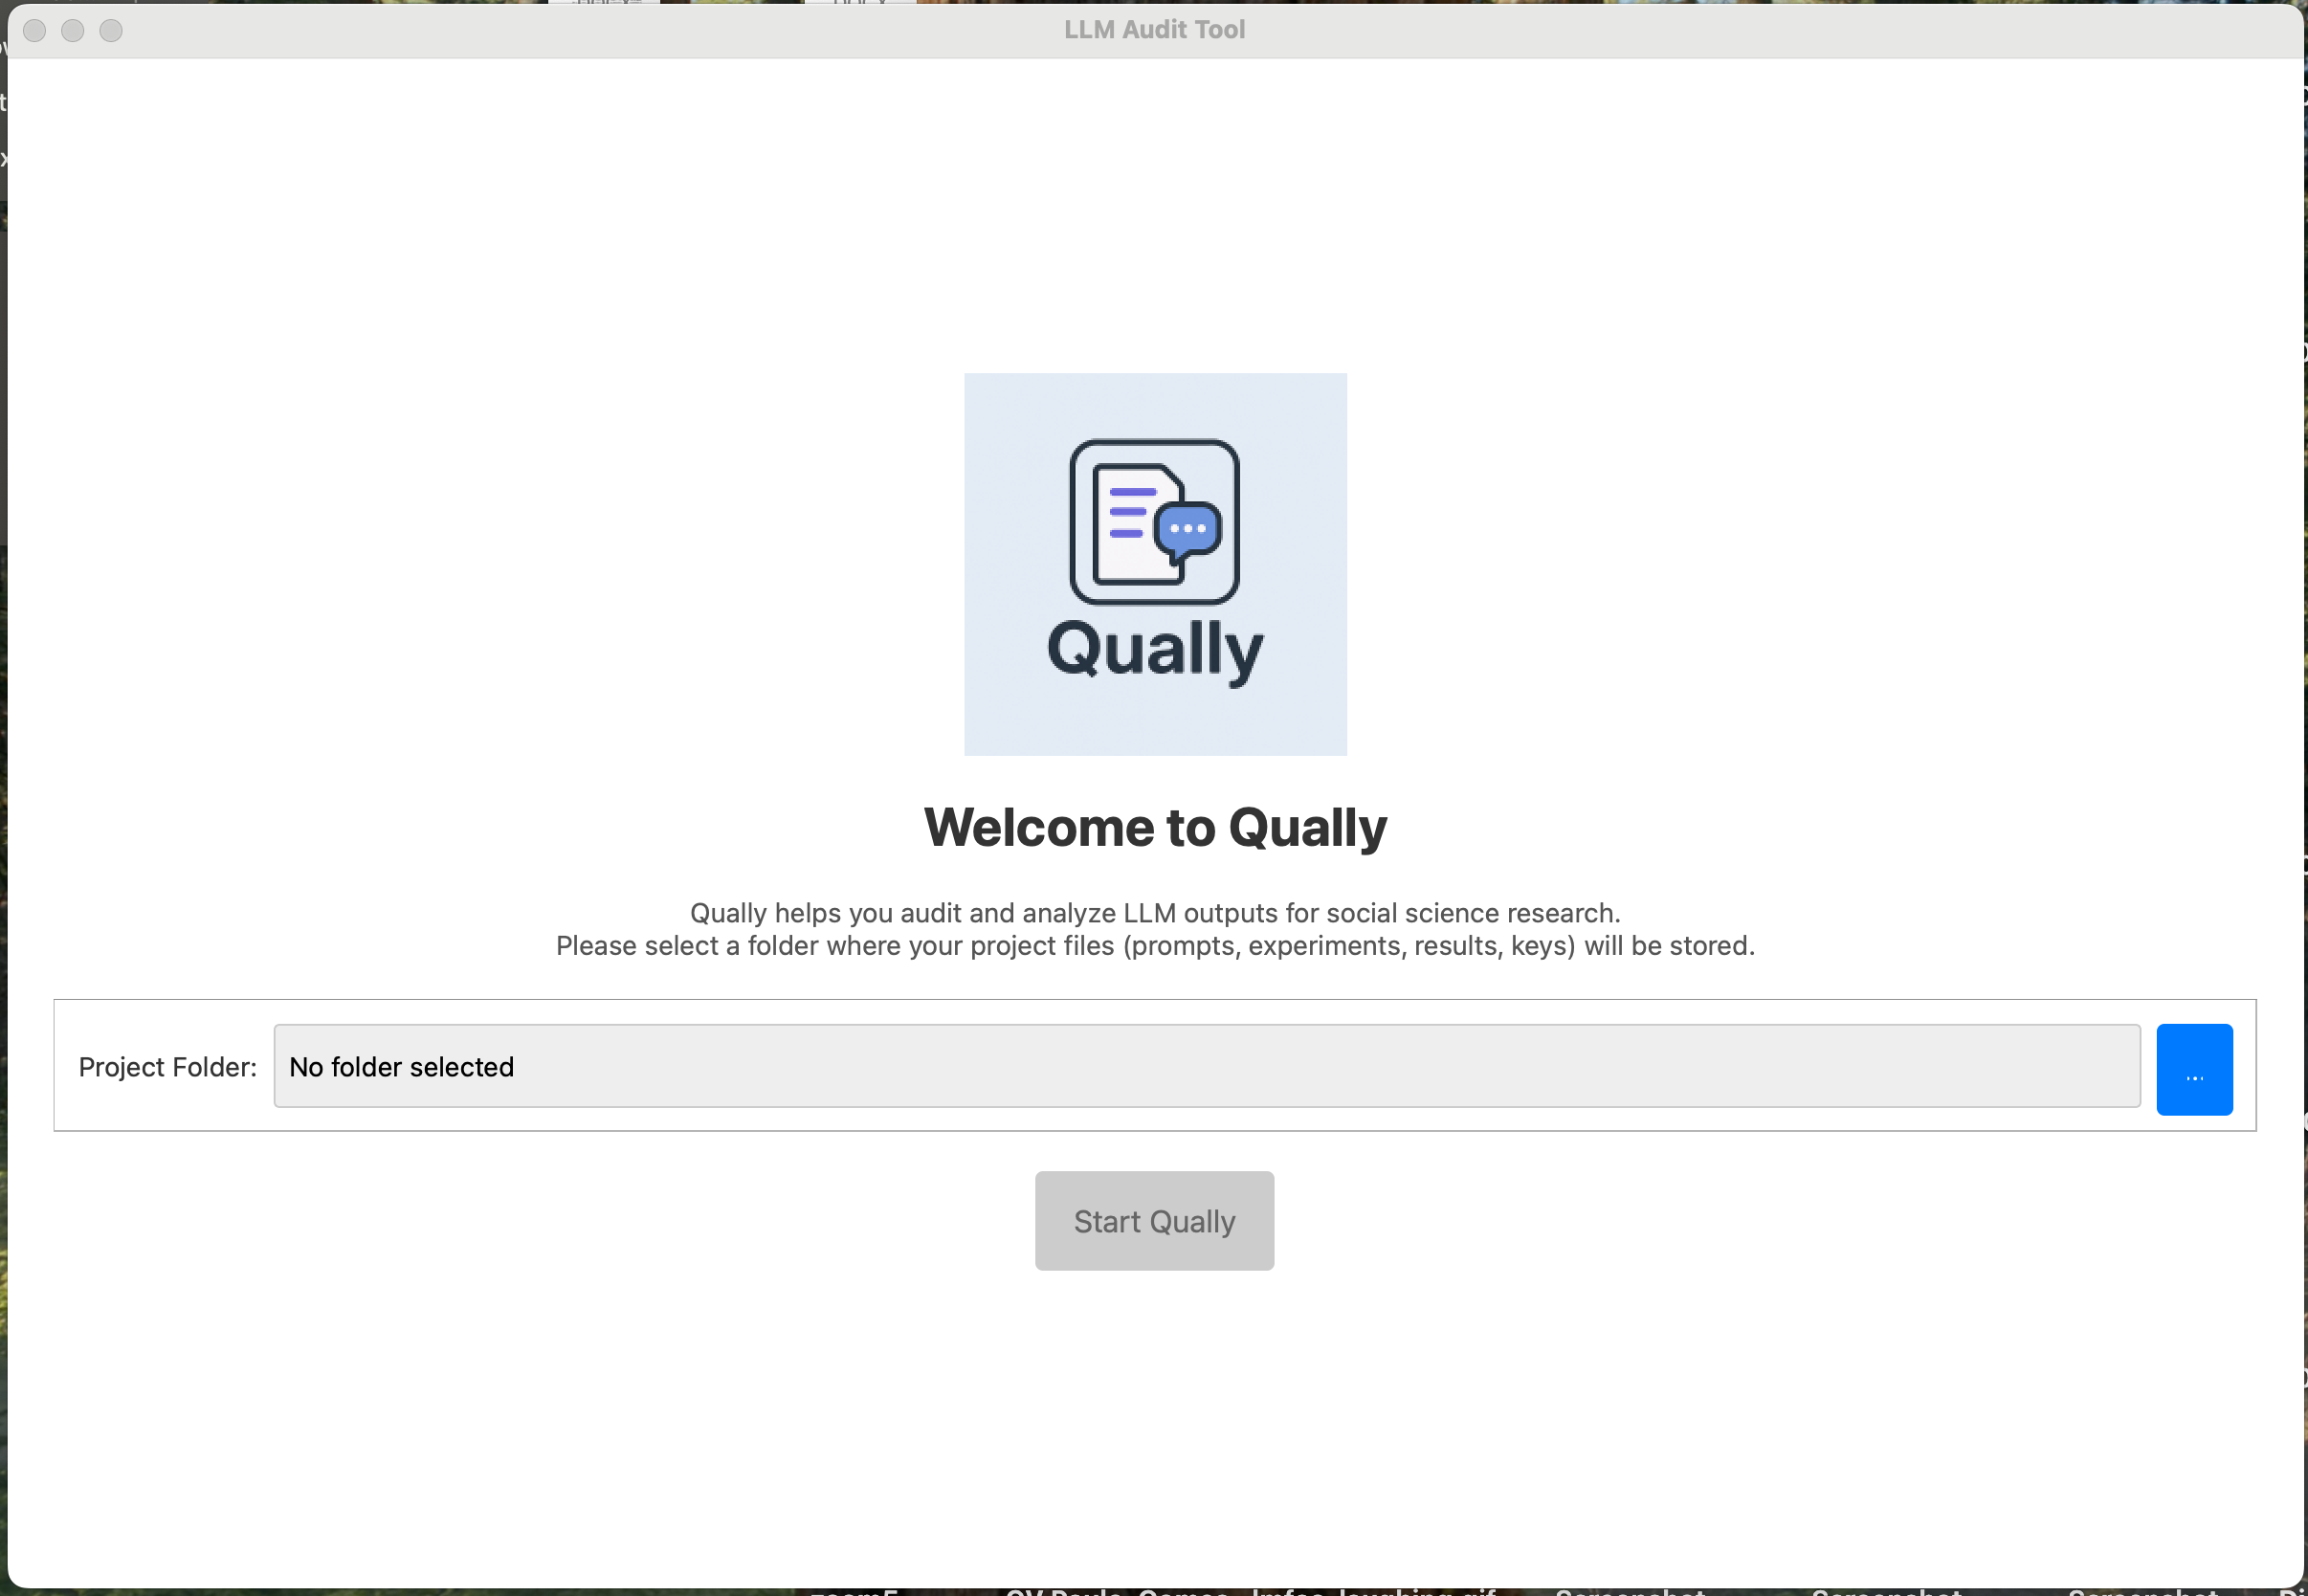
\includegraphics[width=0.9\textwidth]{screenshots/screen1.png}
\caption{Qually Main Interface: Tab-based organization showing API Keys, Data Files, Prompts, Experiments, and Results tabs.}
\label{fig:interface}
\end{figure}

\subsection{Core Components}

\subsubsection{Experiment Manager}

The ExperimentManager class serves as the central coordinator for all experimental activities. It manages:
\begin{itemize}
    \item \textbf{Experiment creation}: Each experiment receives a unique timestamp-based ID and stores metadata including name, description, and creation timestamp
    \item \textbf{Condition management}: Conditions define specific LLM configurations (provider, model, parameters) to test
    \item \textbf{Experiment execution}: Coordinates running prompts across multiple conditions with progress tracking
    \item \textbf{Result storage}: Saves results in structured JSON and CSV formats with timestamps
\end{itemize}

The Experiment Manager uses a project-based organization system, where each project folder contains experiment definitions (\texttt{experiments.json}), prompts, results, and encrypted API keys. This structure enables easy backup, sharing, and version control of research projects.

\subsubsection{Provider Abstraction Layer}

The Provider Abstraction Layer implements a factory pattern to create provider instances dynamically. Each provider (OpenAI, Anthropic, Google, Mistral, Grok, DeepSeek) inherits from a base \texttt{LLMProvider} class that defines a common interface. This abstraction allows researchers to specify experiments in terms of providers and models without needing to know provider-specific API details.

The unified interface includes:
\begin{itemize}
    \item Standardized \texttt{generate()} method that accepts prompt, system prompt, and parameters
    \item Consistent error handling across all providers
    \item Unified response format with text, model, provider, and metadata fields
    \item Automatic parameter mapping from generic names (e.g., "temperature") to provider-specific parameters
\end{itemize}

\subsubsection{API Key Management}

The \texttt{APIKeyManager} class handles secure storage and retrieval of API keys using Fernet encryption (symmetric encryption from the cryptography library). Key features include:

\begin{itemize}
    \item \textbf{Automatic key generation}: Each project generates a unique encryption key on first use
    \item \textbf{Encrypted storage}: API keys are encrypted using Fernet before being stored in \texttt{api\_keys.json}
    \item \textbf{Key isolation}: Each project has its own encryption key, preventing cross-project key access
    \item \textbf{Error handling}: Graceful handling of corrupted or missing encryption keys
\end{itemize}

The encryption key is stored separately in \texttt{encryption\_key.key}, ensuring that even if the encrypted API keys are accessed, they cannot be decrypted without the key file. This two-file approach provides defense in depth for sensitive credentials.

\subsubsection{Rate Limiting System}

The rate limiting system prevents hitting API quotas by implementing configurable delays between requests. Each provider has default rate limits (Table~\ref{tab:providers}), which can be customized in \texttt{settings.json}.

The rate limiting implementation includes:
\begin{itemize}
    \item \textbf{Provider-specific delays}: Different delays for different providers based on their rate limits
    \item \textbf{Thread-safe locking}: Uses threading locks to prevent race conditions in multi-threaded execution
    \item \textbf{Automatic retries}: Implements exponential backoff for HTTP 429 (rate limit) errors
    \item \textbf{Random jitter}: Adds small random delays to prevent thundering herd problems
    \item \textbf{Configurable parameters}: Rates can be adjusted via \texttt{settings.json} without code changes
\end{itemize}

The system uses the \texttt{requests} library's Retry adapter with automatic retries for rate limit errors (HTTP 429) and server errors (5xx), ensuring robust handling of transient API issues.

\section{Features and Capabilities}
\label{sec:features}

\subsection{Multi-Provider Support}

Qually supports six major LLM providers, enabling researchers to compare models across different ecosystems. Each provider is implemented as a separate class inheriting from the base \texttt{LLMProvider} class, ensuring consistent behavior while accommodating provider-specific requirements.

\begin{figure}[ht]
\centering
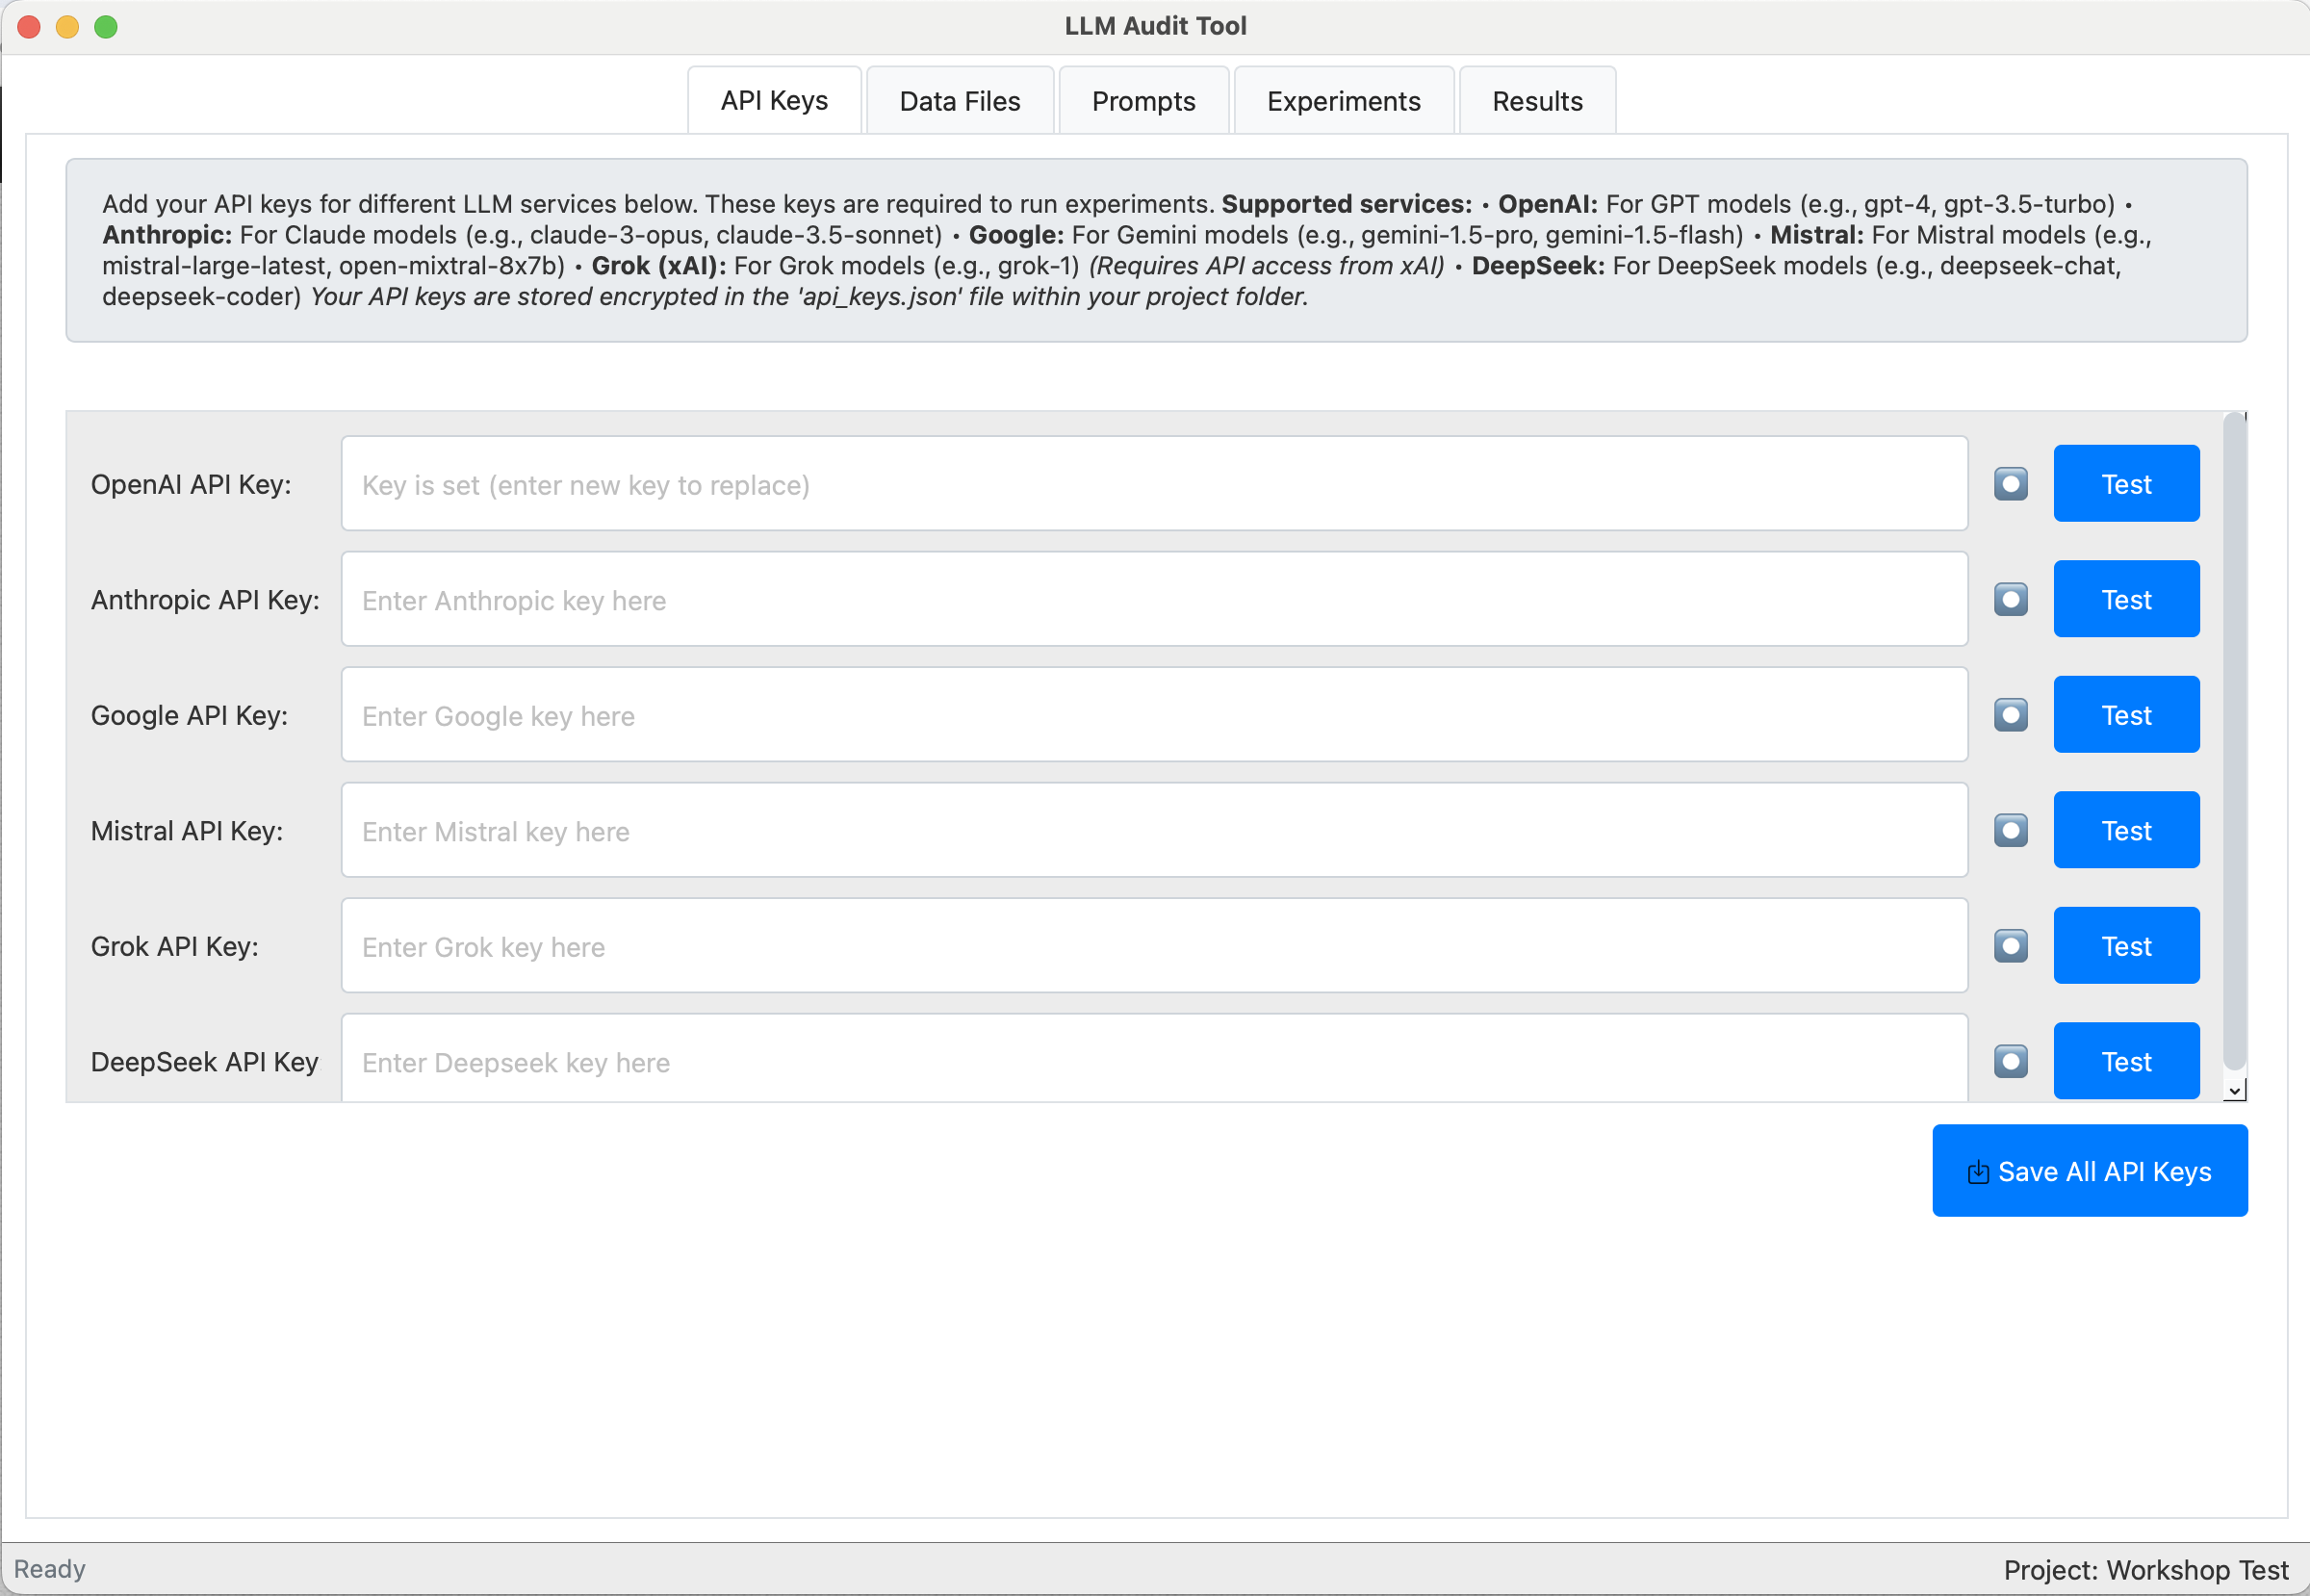
\includegraphics[width=0.9\textwidth]{screenshots/screen2.png}
\caption{API Keys Configuration: Secure API key management interface with encrypted storage for multiple providers.}
\label{fig:apikeys}
\end{figure}

Table~\ref{tab:providers} shows supported providers, example models, and default rate limits. The unified interface means researchers can switch between providers without changing their experimental workflow.

\begin{table}[ht]
\centering
\begin{tabular}{lcc}
\toprule
Provider & Example Models & Default Rate Limit \\
\midrule
OpenAI & gpt-4, gpt-3.5-turbo, gpt-4-turbo & 1.0 req/s \\
Anthropic & claude-3-opus, claude-3.5-sonnet, claude-3-haiku & 0.5 req/s \\
Google & gemini-1.5-pro, gemini-1.5-flash & 0.67 req/s \\
Mistral & mistral-large-latest, open-mixtral-8x7b & 1.0 req/s \\
Grok (xAI) & grok-1 & 1.0 req/s \\
DeepSeek & deepseek-chat, deepseek-coder & 1.0 req/s \\
\bottomrule
\end{tabular}
\caption{Supported LLM Providers and Default Rate Limits}
\label{tab:providers}
\end{table}

\subsection{Experiment Management}

The experiment management system enables researchers to:
\begin{itemize}
    \item \textbf{Create experiments}: Define experiments with names, descriptions, and multiple conditions
    \item \textbf{Add conditions}: Specify different LLM configurations (provider, model, parameters) within a single experiment
    \item \textbf{Select prompts}: Choose which prompts to test in each experiment
    \item \textbf{Run experiments}: Execute experiments with progress tracking and logging
    \item \textbf{View results}: Examine results in tabular format with filtering and sorting
\end{itemize}

\begin{figure}[ht]
\centering
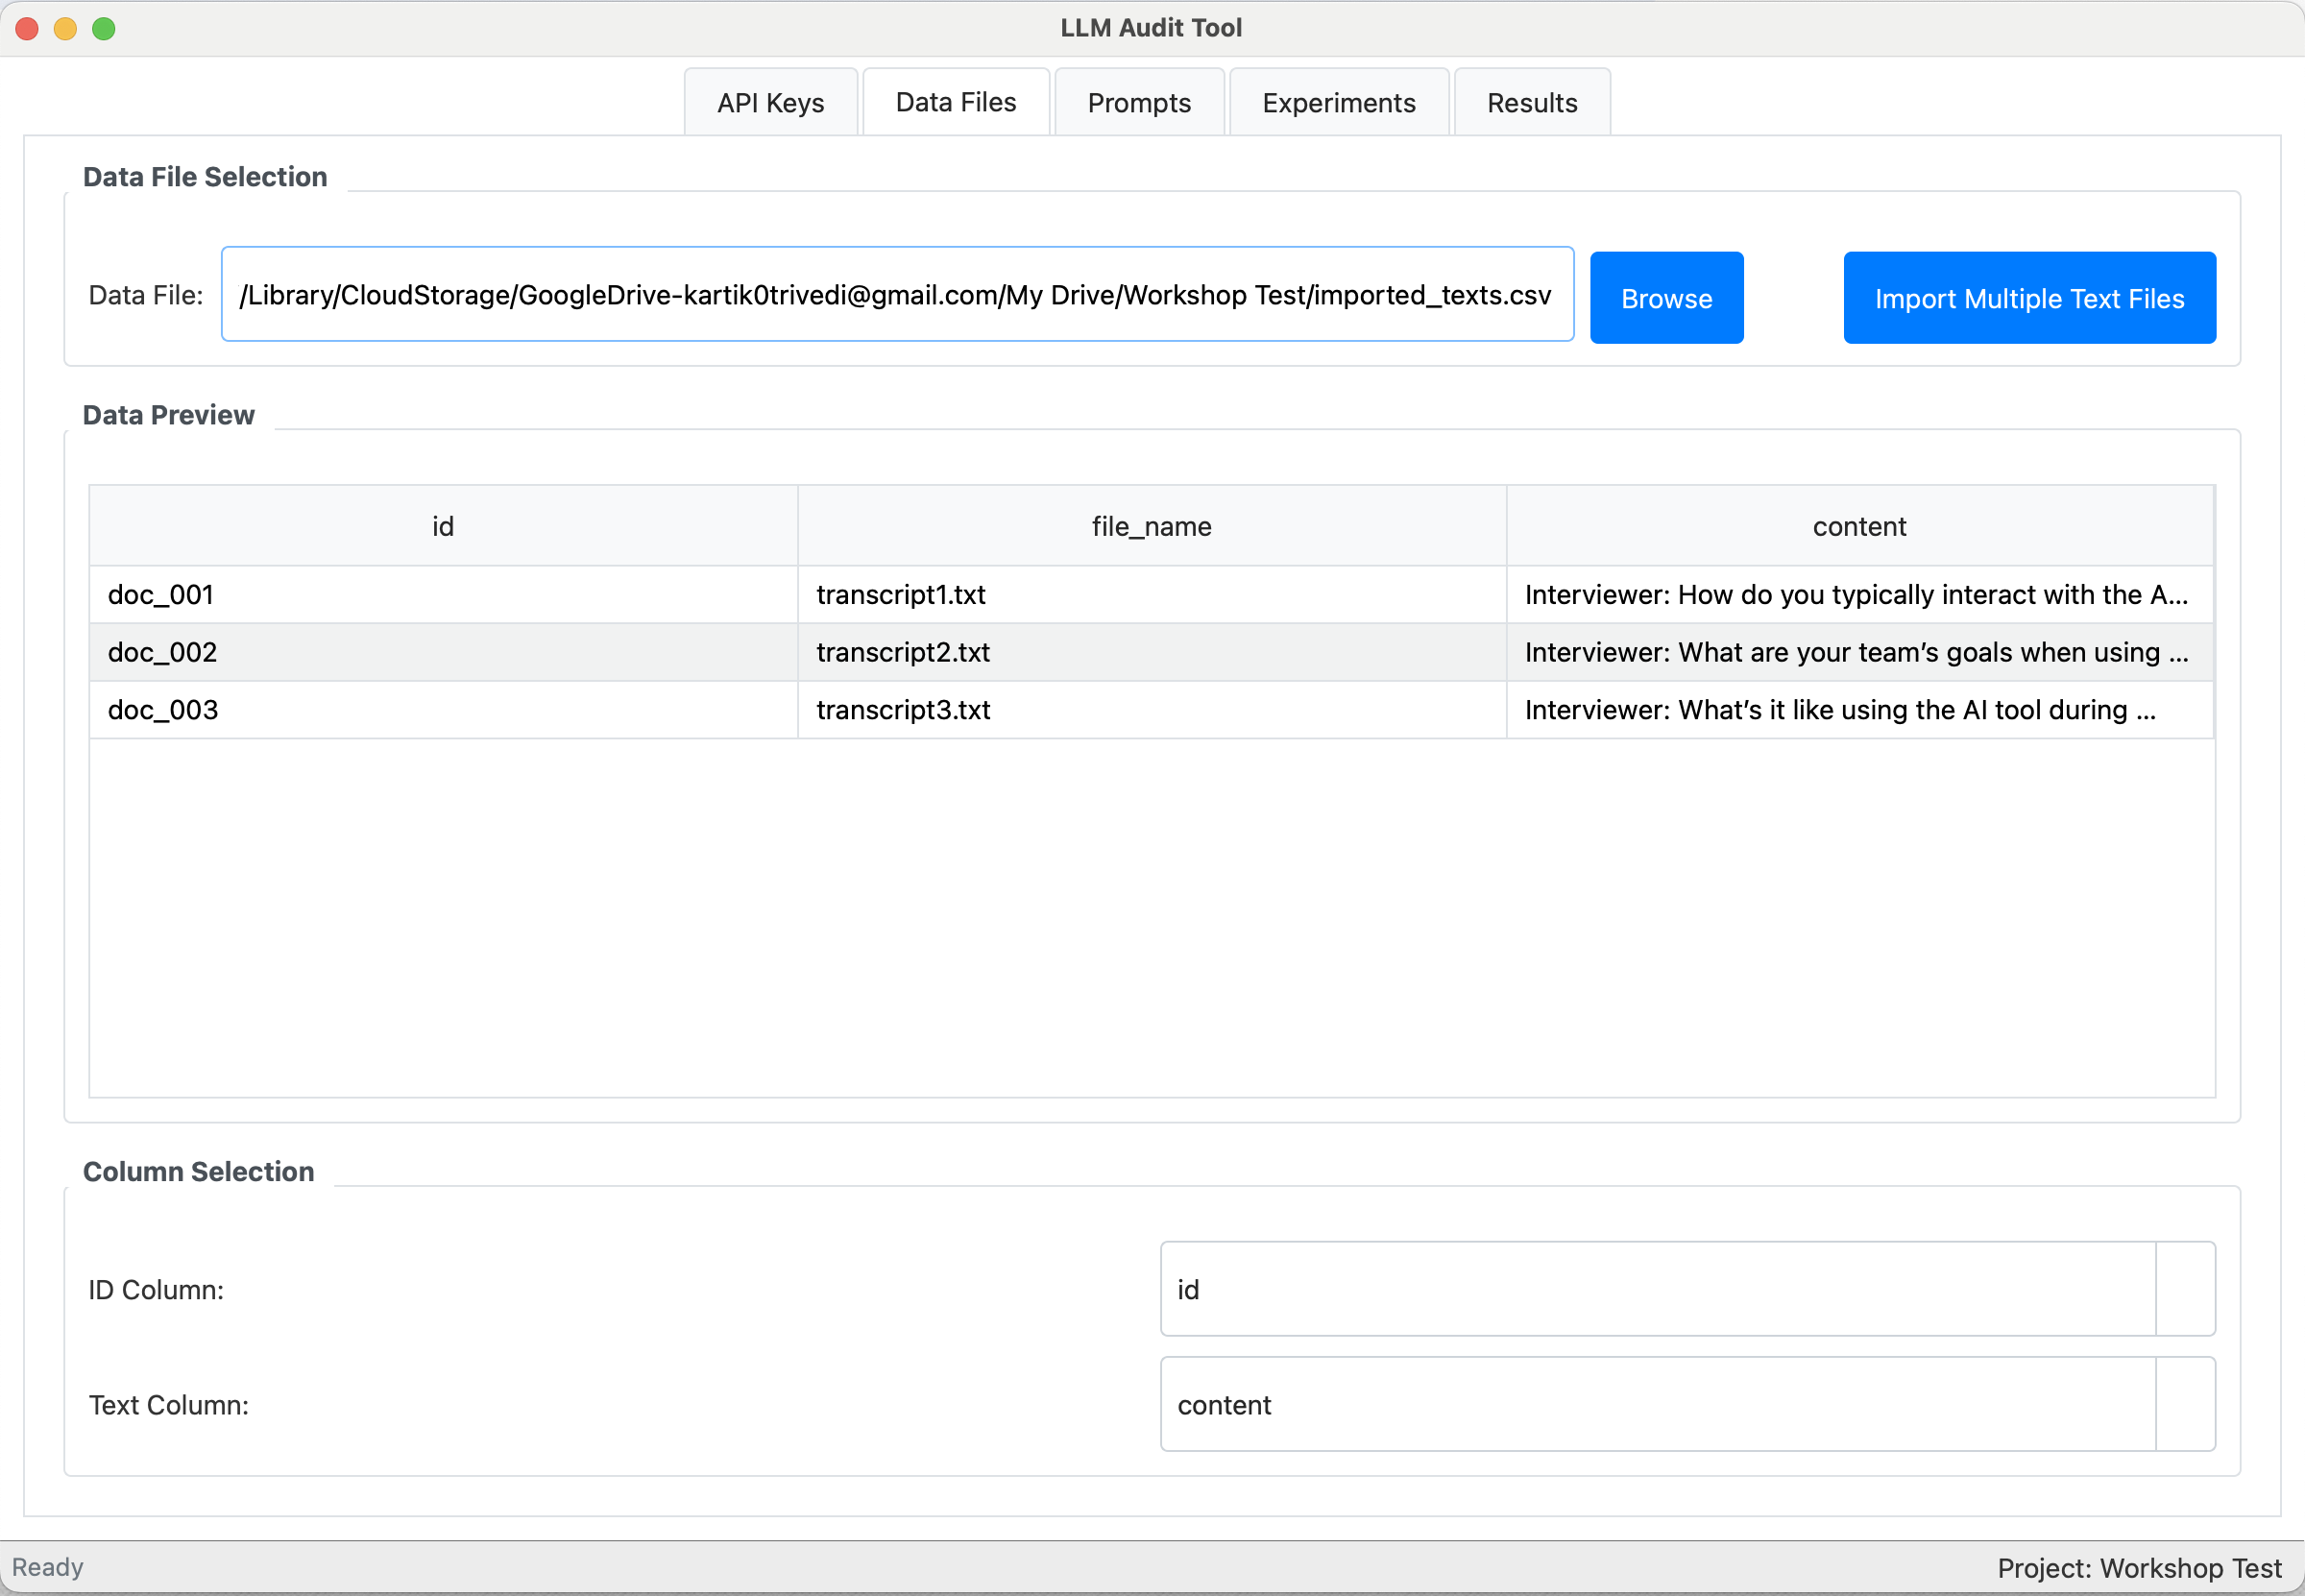
\includegraphics[width=0.9\textwidth]{screenshots/screen3.png}
\caption{Experiment Creation: Interface for creating experiments with multiple conditions, allowing systematic comparison of different LLM configurations.}
\label{fig:experiments}
\end{figure}

Each experiment is assigned a unique ID based on timestamp (\texttt{exp\_<timestamp>}), and conditions receive IDs based on timestamp and sequence (\texttt{cond\_<timestamp>\_<sequence>}). This ensures unique identification while maintaining human-readable timestamps.

\subsection{Data Management}

Qually supports importing prompts and data via CSV files, enabling researchers to work with existing datasets. The data management system includes:

\begin{itemize}
    \item \textbf{CSV import}: Import prompts and metadata from CSV files with automatic column detection
    \item \textbf{Prompt management}: Create, edit, and manage prompts with tags and categories
    \item \textbf{Structured storage}: Prompts stored in CSV format with support for system prompts, tags, and metadata
    \item \textbf{Results export}: Export results in CSV format with all experiment metadata
\end{itemize}

\begin{figure}[ht]
\centering
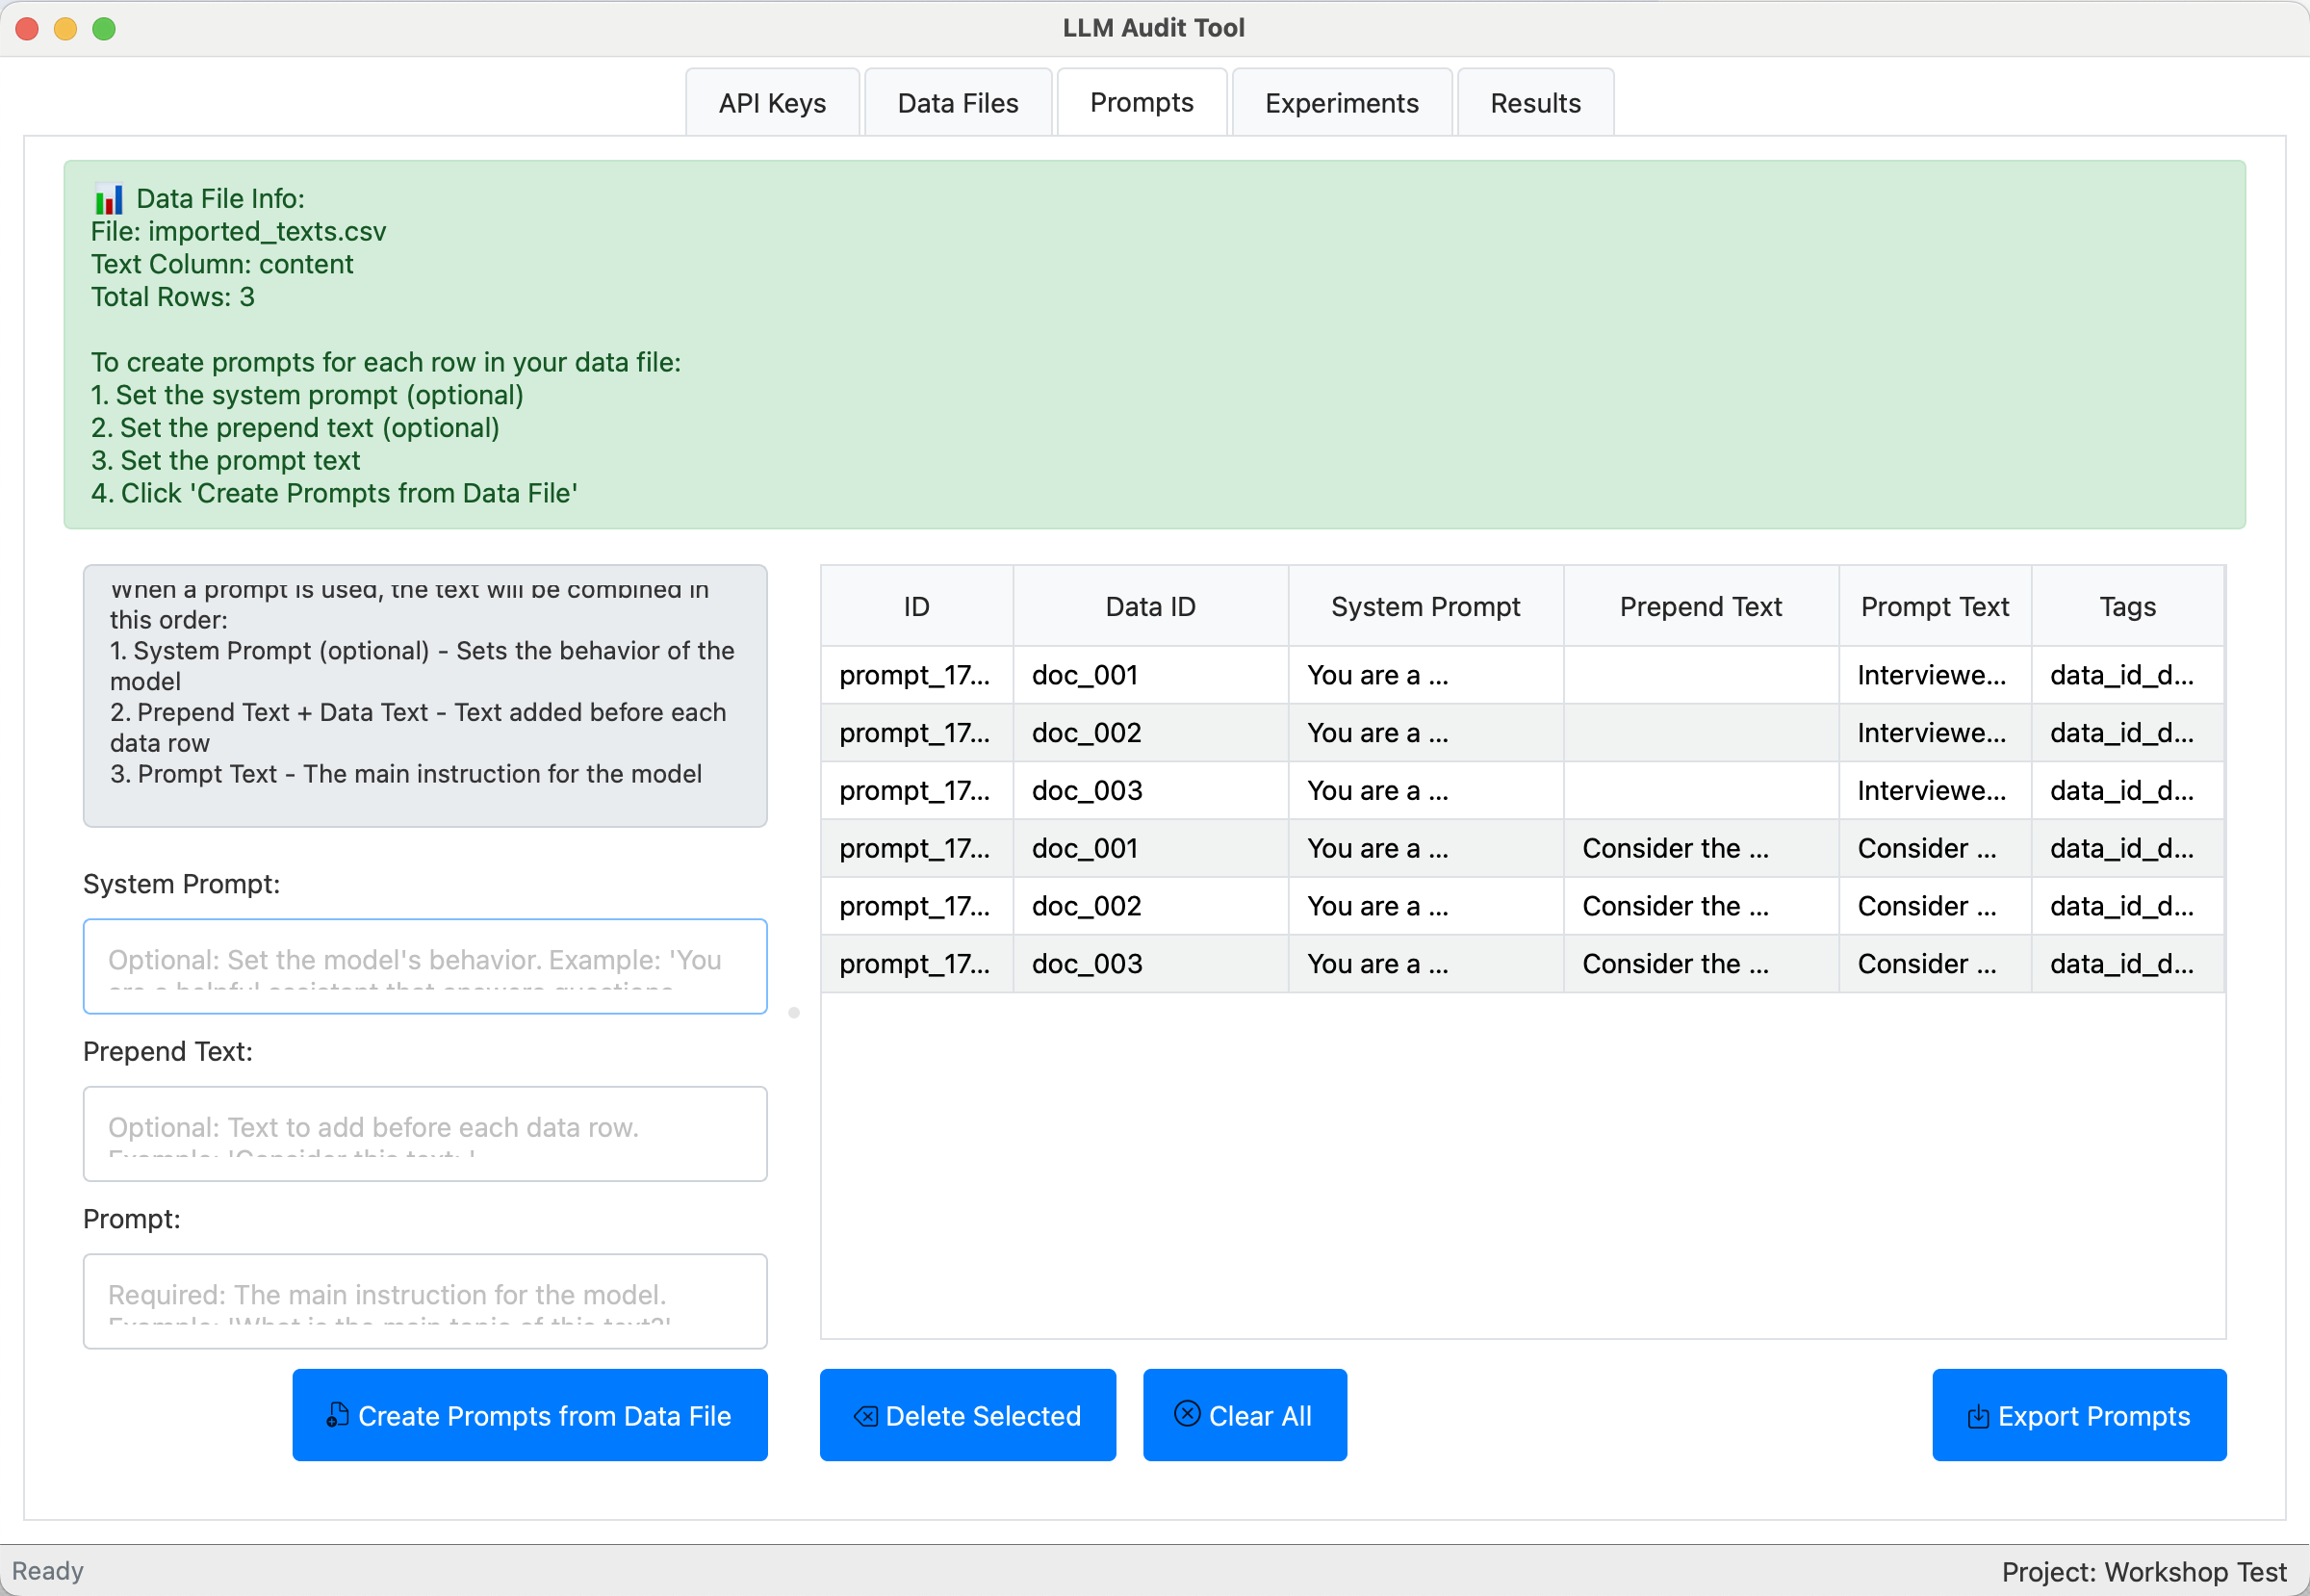
\includegraphics[width=0.9\textwidth]{screenshots/screen4.png}
\caption{Prompt Management: Interface for importing and managing prompts, supporting CSV import and individual prompt creation.}
\label{fig:prompts}
\end{figure}

The prompt management system supports combining prepend text, data text, and prompt text, enabling researchers to create prompts from structured data. This is particularly useful for experiments where prompts need to be generated from datasets.

\subsection{User Interface}

The user interface is organized into five main tabs:
\begin{enumerate}
    \item \textbf{API Keys}: Secure API key management with encryption
    \item \textbf{Data Files}: CSV import and data file management
    \item \textbf{Prompts}: Prompt creation, editing, and management
    \item \textbf{Experiments}: Experiment creation and execution
    \item \textbf{Results}: Results viewing, filtering, and export
\end{enumerate}

The interface includes:
\begin{itemize}
    \item \textbf{Progress tracking}: Progress bars and log messages during experiment execution
    \item \textbf{Error handling}: User-friendly error messages and validation
    \item \textbf{Status bar}: Shows current project and application status
    \item \textbf{Responsive design}: Interface remains responsive during long-running experiments
\end{itemize}

\begin{figure}[ht]
\centering
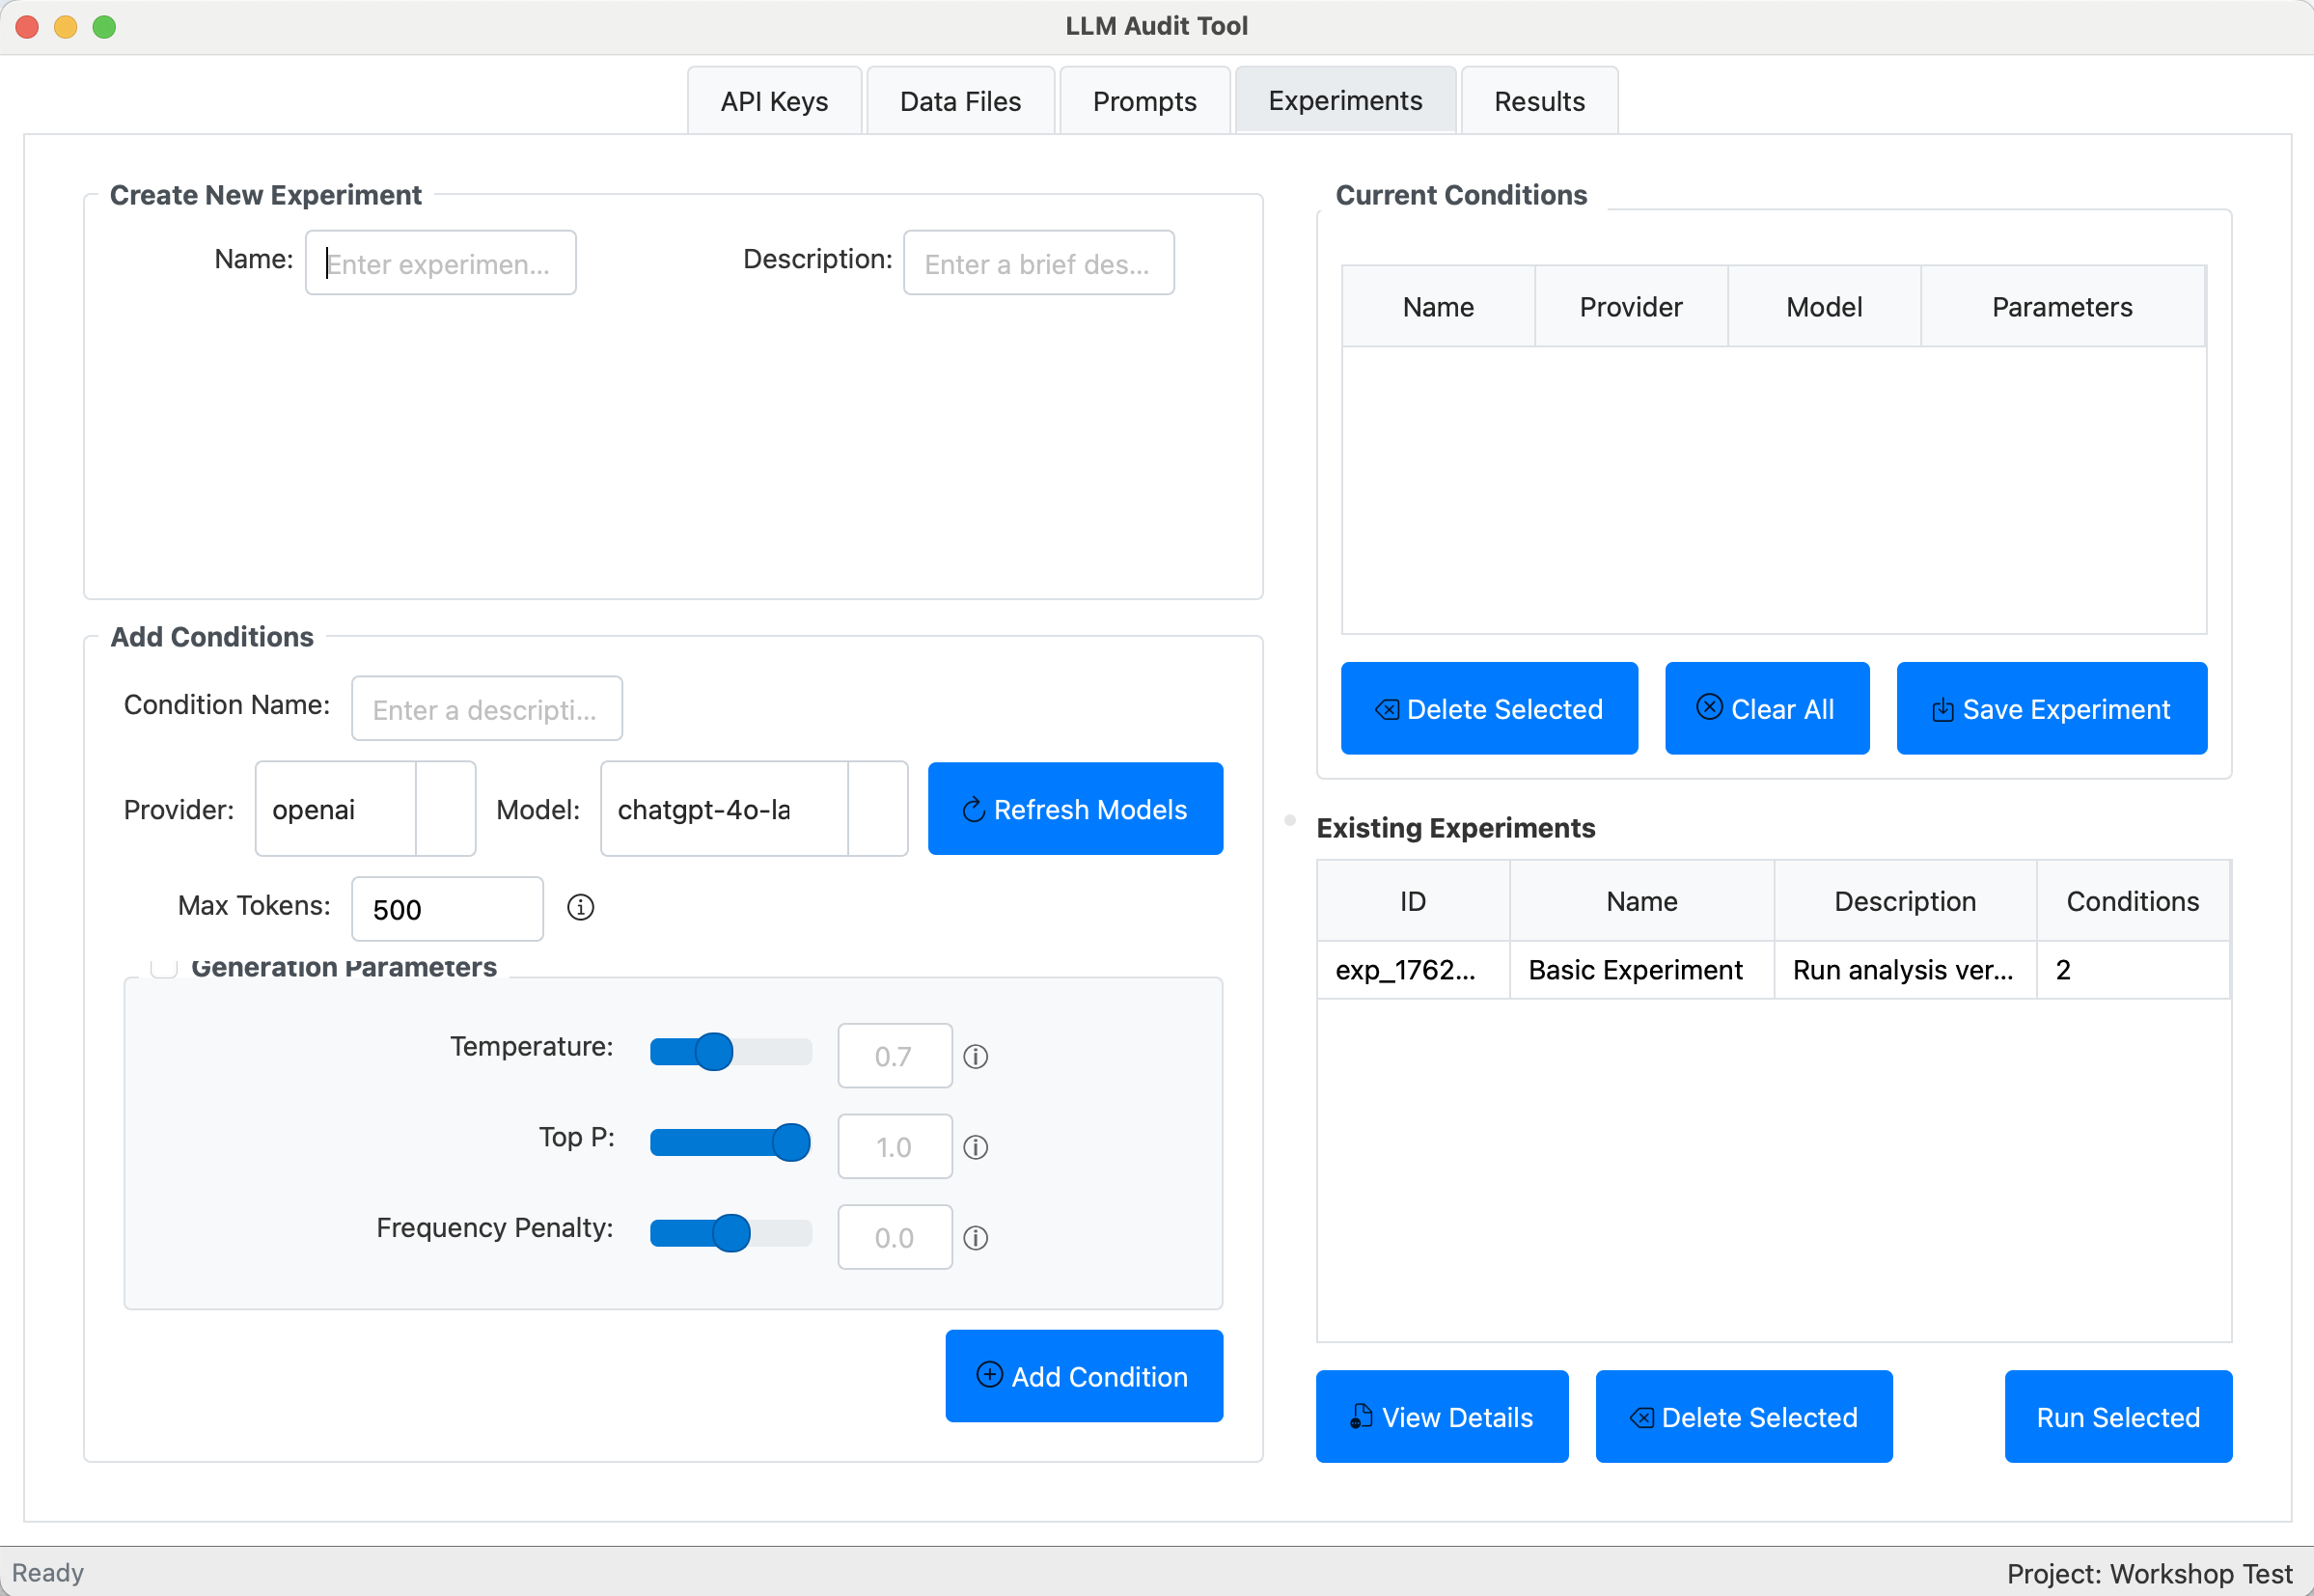
\includegraphics[width=0.9\textwidth]{screenshots/screen5.png}
\caption{Results View: Table interface for viewing, filtering, and exporting experimental results with support for multiple experiments and conditions.}
\label{fig:results}
\end{figure}

\section{Use Cases and Examples}
\label{sec:use_cases}

\subsection{Use Case 1: Bias Evaluation}

A researcher wants to evaluate gender bias in LLM responses to job-related prompts. Using Qually, they:

\begin{enumerate}
    \item Import a CSV file containing prompts with gender-neutral job descriptions
    \item Create an experiment with three conditions:
    \begin{itemize}
        \item Condition 1: GPT-4 with temperature=0.7
        \item Condition 2: Claude-3.5-Sonnet with temperature=0.7
        \item Condition 3: Gemini-1.5-Pro with temperature=0.7
    \end{itemize}
    \item Run the experiment and export results to CSV
    \item Analyze responses for gender bias indicators
\end{enumerate}

This workflow enables systematic comparison of bias across providers using identical prompts, ensuring fair comparison.

\subsection{Use Case 2: Prompt Engineering Study}

A researcher wants to test different prompt formulations to optimize LLM performance on a specific task. They:

\begin{enumerate}
    \item Create multiple prompt variations (e.g., with/without examples, different instructions)
    \item Set up an experiment with multiple conditions varying prompt structure
    \item Run the experiment across multiple models
    \item Compare performance metrics across prompt formulations
\end{enumerate}

Qually's condition system allows testing multiple prompt variations and model configurations in a single experiment, streamlining prompt engineering workflows.

\subsection{Use Case 3: Model Comparison}

A researcher wants to compare responses from different models to the same set of prompts for a systematic evaluation. They:

\begin{enumerate}
    \item Create an experiment with conditions for each model they want to compare
    \item Select all prompts to test
    \item Run the experiment and monitor progress
    \item Export results for statistical analysis
\end{enumerate}

\begin{figure}[ht]
\centering
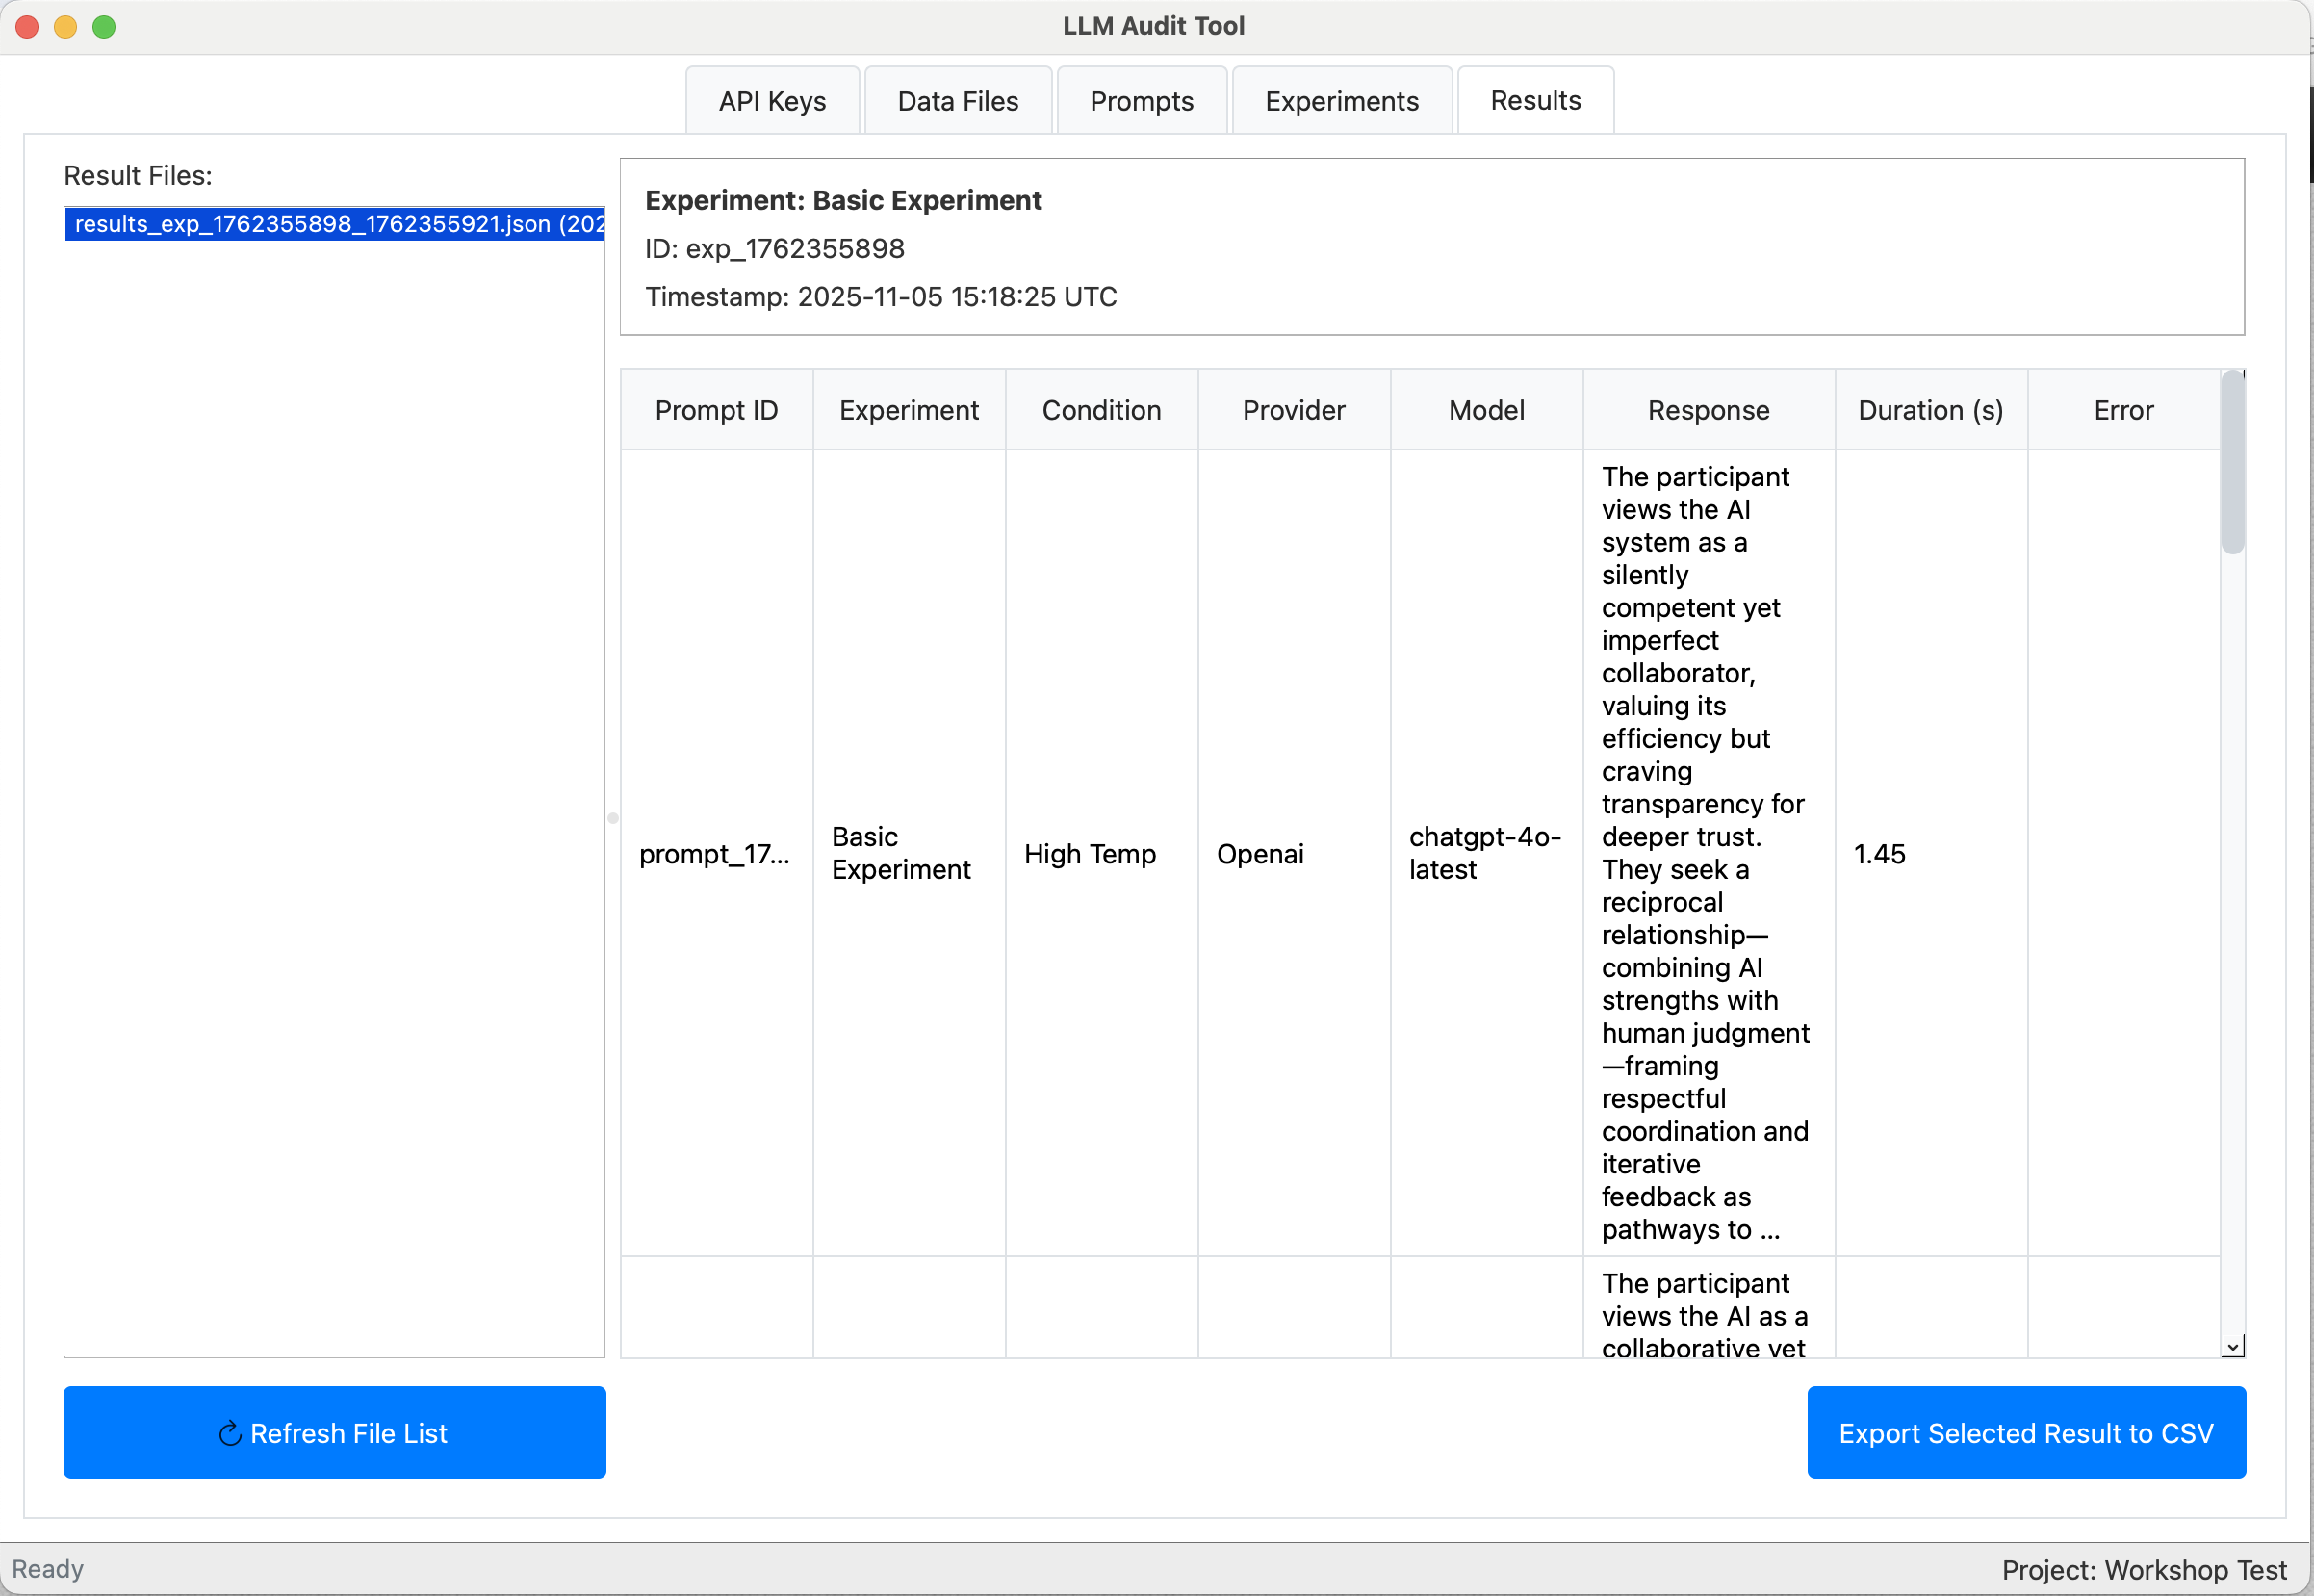
\includegraphics[width=0.9\textwidth]{screenshots/screen6.png}
\caption{Experiment Execution: Real-time progress tracking during experiment execution with log messages and progress indicators.}
\label{fig:execution}
\end{figure}

This use case demonstrates Qually's strength in enabling systematic, reproducible comparisons across multiple models and providers.

\section{Technical Details}
\label{sec:technical}

\subsection{Implementation}

Qually is implemented in Python 3.11+ using the following key technologies:

\begin{itemize}
    \item \textbf{PyQt6} ($\geq$6.9.0): GUI framework for cross-platform desktop application
    \item \textbf{pandas} ($\geq$2.2.0): Data manipulation for CSV import/export
    \item \textbf{requests} ($\geq$2.32.0): HTTP library for API calls with retry support
    \item \textbf{cryptography} ($\geq$44.0.0): Encryption library for API key security
\end{itemize}

The application is structured as a single-file GUI (\texttt{qually\_gui.py}) and core logic module (\texttt{qually\_tool.py}), enabling easy distribution and maintenance. The codebase follows object-oriented design principles with clear separation between GUI logic and business logic.

Qually supports both development mode (running directly from source) and packaged applications for macOS (using py2app) and Windows (using PyInstaller). The project structure is designed to be self-contained, with all project data stored in user-specified project folders.

\subsection{Rate Limiting}

The rate limiting system implements provider-specific delays to prevent hitting API quotas. Default delays are conservative and based on typical API limits:

\begin{itemize}
    \item \textbf{OpenAI}: 1.0 second delay (60 requests/minute limit)
    \item \textbf{Anthropic}: 2.0 second delay (more conservative for Claude API)
    \item \textbf{Google}: 1.5 second delay (40 requests/minute limit)
    \item \textbf{Other providers}: 1.0 second delay
\end{itemize}

The system uses threading locks to ensure thread-safe rate limiting, and implements exponential backoff with jitter for handling rate limit errors. Rate limits can be configured via \texttt{settings.json} without modifying code.

The retry mechanism uses the \texttt{urllib3} Retry adapter with:
\begin{itemize}
    \item Maximum 3 retries
    \item Exponential backoff (0.5s, 1s, 2s)
    \item Retry on HTTP 429 (rate limit) and 5xx (server errors)
    \item Random jitter to prevent synchronized retries
\end{itemize}

\subsection{Security}

API key security is implemented using Fernet symmetric encryption from the Python cryptography library. Fernet is a high-level interface built on top of AES-128 in CBC mode with HMAC-SHA256 for authentication.

Key security features:
\begin{itemize}
    \item \textbf{Automatic key generation}: Each project generates a unique 256-bit encryption key
    \item \textbf{Separate key storage}: Encryption key stored in separate file (\texttt{encryption\_key.key})
    \item \textbf{Encrypted storage}: API keys encrypted before storage in \texttt{api\_keys.json}
    \item \textbf{Key isolation}: Each project has its own encryption key
    \item \textbf{No key transmission}: Keys never transmitted over network
\end{itemize}

The encryption key is generated using \texttt{cryptography.fernet.Fernet.generate\_key()}, which uses \texttt{os.urandom()} for cryptographically secure random number generation. The key is stored in binary format and never logged or displayed.

API keys are only decrypted in memory when needed for API calls, and are never stored in plaintext. This ensures that even if project files are accessed, API keys remain protected unless the attacker has both the encrypted keys file and the encryption key file.

\section{User Manual and Documentation}
\label{sec:manual}

A comprehensive user manual for Qually is available as a separate document. The user manual provides detailed, step-by-step instructions for:

\begin{itemize}
    \item Installation and setup procedures
    \item Creating and managing projects
    \item Adding and securing API keys
    \item Importing data and creating prompts
    \item Setting up and running experiments
    \item Managing multiple conditions and providers
    \item Viewing and exporting results
    \item Troubleshooting common issues
    \item Best practices for reproducible research
\end{itemize}

The user manual is available at: \url{https://github.com/kartik0trivedi/Qually} (see \texttt{documentation/qually\_user\_manual.pdf}).

For quick reference, basic installation steps are:
\begin{enumerate}
    \item Clone the repository: \texttt{git clone https://github.com/kartik0trivedi/Qually.git}
    \item Install dependencies: \texttt{pip install -r requirements.txt}
    \item Run the application: \texttt{python qually\_gui.py}
\end{enumerate}

Detailed usage instructions, troubleshooting guides, and examples are provided in the comprehensive user manual.

\section{Limitations and Future Work}
\label{sec:limitations}

\subsection{Current Limitations}

Qually has several current limitations:

\begin{itemize}
    \item \textbf{Provider-specific differences}: Different providers have different parameter names and ranges, which may require manual adjustment
    \item \textbf{Rate limiting trade-offs}: Conservative rate limits may slow down large experiments, but can be adjusted in settings
    \item \textbf{GUI limitations}: Advanced features may require understanding the underlying data structures
    \item \textbf{Single-threaded execution}: Experiments run sequentially, which may be slow for very large experiments
    \item \textbf{No built-in analysis}: Results export is provided, but statistical analysis must be done in external tools
\end{itemize}

\subsection{Future Enhancements}

Planned future enhancements include:

\begin{itemize}
    \item \textbf{Additional providers}: Support for additional LLM providers (e.g., Cohere, Together AI)
    \item \textbf{Advanced analysis}: Built-in statistical analysis and visualization tools
    \item \textbf{Batch processing}: Parallel execution of experiments across multiple threads
    \item \textbf{Template system}: Pre-built experiment templates for common use cases
    \item \textbf{Integration with analysis tools}: Direct integration with R and Python analysis pipelines
    \item \textbf{Cloud sync}: Optional cloud synchronization for project backup
    \item \textbf{Advanced filtering}: More sophisticated result filtering and search capabilities
\end{itemize}

\section{Discussion and Implications}
\label{sec:discussion}

\subsection{Impact on Social Science Research}

Qually has the potential to significantly impact social science research by:

\begin{itemize}
    \item \textbf{Democratizing LLM evaluation}: Making systematic LLM auditing accessible to researchers without programming expertise
    \item \textbf{Enabling systematic audits}: Providing tools for rigorous, reproducible evaluation of LLM behavior
    \item \textbf{Supporting reproducibility}: Structured data export and experiment tracking enable reproducible research
    \item \textbf{Facilitating comparison}: Enabling easy comparison of models across different providers
\end{itemize}

By removing technical barriers, Qually enables more researchers to conduct systematic LLM evaluations, potentially improving the quality and rigor of LLM-based research in the social sciences.

\subsection{Methodological Considerations}

When using Qually for research, several methodological considerations are important:

\begin{itemize}
    \item \textbf{Experimental design}: Researchers should carefully design experiments to ensure fair comparison across conditions
    \item \textbf{Parameter consistency}: When comparing models, ensure parameters are comparable across providers
    \item \textbf{Reproducibility}: Document all experimental conditions, including model versions and parameters
    \item \textbf{Sampling}: Consider prompt sampling strategies for large-scale evaluations
    \item \textbf{Analysis}: Use appropriate statistical methods for comparing results across conditions
\end{itemize}

Qually's structured export format facilitates these methodological considerations by ensuring all experimental details are captured and can be reviewed.

\section{Conclusion}
\label{sec:conclusion}

We have presented Qually, a GUI-based tool for conducting systematic LLM audits in social science research. Qually addresses the gap between powerful but technically complex LLM evaluation frameworks and the needs of social science researchers by providing an accessible, user-friendly interface for conducting experiments across multiple LLM providers.

Key contributions include:
\begin{itemize}
    \item First GUI-based tool specifically designed for LLM auditing in social science
    \item Unified interface for multiple LLM providers
    \item Integrated experiment management with automatic tracking
    \item Secure API key management with encryption
    \item Built-in rate limiting to prevent API quota issues
    \item Structured data export for reproducible research
\end{itemize}

Qually enables researchers without programming expertise to conduct systematic LLM evaluations, potentially improving the quality and accessibility of LLM-based research in the social sciences. The tool is freely available and open-source, enabling the research community to contribute improvements and extensions.

We encourage researchers to use Qually for their LLM auditing needs and welcome feedback and contributions to improve the tool.

\section*{Acknowledgments}
Funding for this application was provided by the Advanced Rehabilitation Research and Training (ARRT) Program on Employment at the University of New Hampshire, which is funded by the National Institute for Disability, Independent Living, and Rehabilitation Research, in the Administration for Community Living, at the U.S. Department of Health and Human Services (DHHS) under grant number 90AREM000401. The contents do not necessarily represent the policy of DHHS and you should not assume endorsement by the federal government (EDGAR, 75.620 (b)).

\begin{thebibliography}{99}
\bibitem{github} Qually GitHub Repository. \url{https://github.com/kartik0trivedi/Qually}
\end{thebibliography}

\end{document}
